\chapter{Time series: stationarity and autocorrelation}
\label{cap:est}

\section{Why time series need their own tools}
In cross-section data, independent observations are reasonable. In a series, today's value depends on yesterday's. This changes everything: the same series is our only sample, and we can only learn from it if its behavior is, in some sense, stable over time. That stability has a name: \textbf{stationarity}.

\section{Weak stationarity}
A series $\{y_t\}$ is \textbf{weakly stationary} (or covariance stationary) if
\begin{enumerate}[leftmargin=1.6em]
\item $\E(y_t)=\mu$ does not depend on $t$;
\item $\Var(y_t)=\gamma_0$ does not depend on $t$;
\item $\Cov(y_t,y_{t-k})=\gamma_k$ depends only on the lag $k$, not on $t$.
\end{enumerate}
The \textbf{autocorrelation function} (ACF) is $\rho_k=\gamma_k/\gamma_0$. The \textbf{partial ACF} (PACF) at $k$ is the correlation between $y_t$ and $y_{t-k}$ after removing the effect of the intermediate lags.

\begin{intuicao}[ACF versus PACF]
The ACF mixes direct and indirect effects: if today depends on yesterday and yesterday on the day before, today and two days ago are correlated even without a direct link. The PACF tries to isolate only the direct link.
\end{intuicao}

\section{Four series you need to know}
\begin{center}
\small
\begin{tabular}{p{3.2cm}p{4.1cm}p{6.4cm}}
\toprule
\textbf{Series} & \textbf{Definition} & \textbf{Properties} \\
\midrule
White noise & $y_t=\varepsilon_t$, mean 0, variance $\sigma^2$, uncorrelated & $\rho_k=0$ for $k\ge1$. Building block of all models. \\
Random walk & $y_t=y_{t-1}+\varepsilon_t$ & \textbf{Not} stationary: the variance $t\sigma^2$ grows. Shocks are permanent. \\
AR(1) & $y_t=\phi y_{t-1}+\varepsilon_t$ & Stationary if $|\phi|<1$; $\rho_k=\phi^k$ (geometric decay). \\
MA(1) & $y_t=\varepsilon_t+\theta\varepsilon_{t-1}$ & Always stationary; $\rho_1=\theta/(1+\theta^2)$ and $\rho_k=0$ for $k\ge2$. \\
\bottomrule
\end{tabular}
\end{center}

\begin{atencao}[Pitfall: the sign of the MA changes from book to book]
This guide uses $y_t=\varepsilon_t+\theta\varepsilon_{t-1}$ (\textbf{positive} sign), like Hamilton, R's \texttt{arima} and \texttt{statsmodels}. Cryer and Chan and Mills use the \textbf{negative} sign, $y_t=\varepsilon_t-\theta\varepsilon_{t-1}$, inherited from Box and Jenkins. With the negative convention, $\rho_1=-\theta/(1+\theta^2)$. If you copy a formula from a book and a coefficient from a software package without checking the convention, the sign of $\theta$ comes out reversed. When reading software output, always confirm which convention it uses.
\end{atencao}

\begin{simulacao}[Checked: MA(1) with coefficient 0.5]
The formula gives $\rho_1=0.5/1.25=0.4$. The theoretical autocorrelation computed by \texttt{statsmodels} is $0.4$. Note also that $\theta=2$ gives $2/5=0.4$: \textbf{two values of $\theta$ (one and its inverse) generate the same ACF}. That is why invertibility, $|\theta|<1$, is required to identify the model. And the maximum of $|\rho_1|$ in an MA(1) is $0.5$.
\end{simulacao}

\section{AR(2) and the stationarity condition}
For $y_t=\phi_1y_{t-1}+\phi_2y_{t-2}+\varepsilon_t$, the three conditions below are equivalent to ``roots of the polynomial outside the unit circle'' (the so-called stationarity triangle):
\[
\phi_1+\phi_2<1,\qquad \phi_2-\phi_1<1,\qquad |\phi_2|<1.
\]
The Yule--Walker equations give $\rho_1=\phi_1/(1-\phi_2)$ and $\rho_k=\phi_1\rho_{k-1}+\phi_2\rho_{k-2}$ for $k\ge2$.

\begin{simulacao}[Checked: AR(2) with coefficients 0.5 and 0.3]
Yule--Walker: $\rho_1=0.5/0.7=0.7143$ and $\rho_2=0.5\times0.7143+0.3=0.6571$. \texttt{statsmodels} gives the same values. I also tested five pairs $(\phi_1,\phi_2)$ by computing the roots: $(0.5;0.3)$ is stationary; $(1.2;-0.2)$, $(0.5;0.6)$, $(1.0;0)$ and $(-0.5;0.5)$ are not, which matches the triangle.
\end{simulacao}

\section{Signatures in the ACF and PACF}
\begin{center}
\small
\begin{tabular}{lcc}
\toprule
\textbf{Model} & \textbf{ACF} & \textbf{PACF} \\
\midrule
AR($p$) & decays gradually & \textbf{cuts off} after $p$ \\
MA($q$) & \textbf{cuts off} after $q$ & decays gradually \\
ARMA($p,q$) & decays & decays \\
\bottomrule
\end{tabular}
\end{center}

\begin{center}
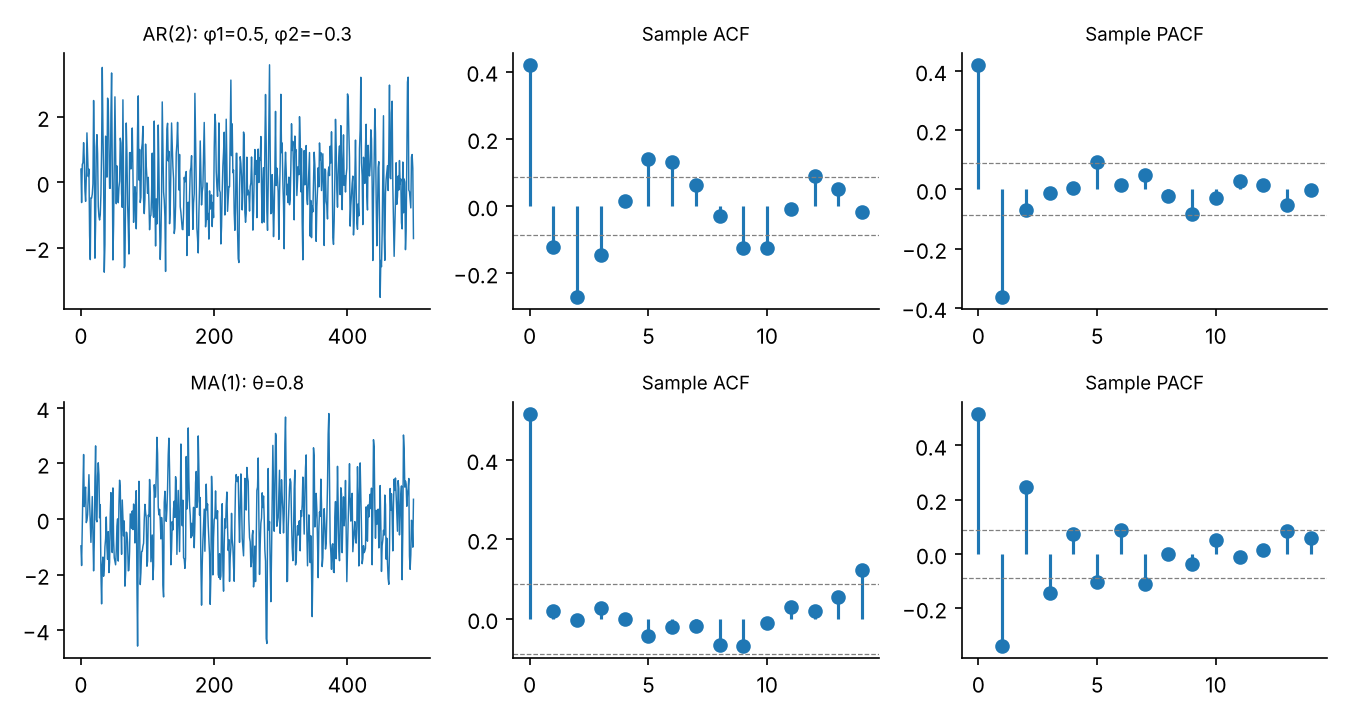
\includegraphics[width=\textwidth]{fig/acf_pacf.png}\\
\small Simulated series (500 points) and their sample ACF and PACF. Top row: AR(2) ($\phi_1=0.5$, $\phi_2=-0.3$): the PACF cuts off at 2. Bottom row: MA(1) ($\theta=0.8$): the ACF cuts off at 1. Dotted lines are the $\pm1.96/\sqrt n$ bands.
\end{center}

\begin{atencao}
The $\pm1.96/\sqrt n$ bands hold under the white-noise hypothesis. For a series that is \emph{not} white noise, the correct (Bartlett) bands are wider, and in short samples the sample ACF is biased downward. Interpret the plots as a clue, not a verdict.
\end{atencao}

\begin{exercicio}
In an AR(1) with $\phi=0.6$ and $\sigma^2=1$, compute $\gamma_0$, $\rho_1$ and $\rho_3$.
\end{exercicio}
\sol{$\gamma_0=\sigma^2/(1-\phi^2)=1/0.64=1.5625$. $\rho_1=0.6$ and $\rho_3=0.6^3=0.216$.}

\begin{exercicio}
An MA(1) has $\theta=-0.4$ (positive convention). What is $\rho_1$? And if the book's convention were the negative one, with the same number $-0.4$ printed?
\end{exercicio}
\sol{Positive convention: $\rho_1=-0.4/(1+0.16)=-0.345$. Negative convention, with $\theta=-0.4$: $\rho_1=-\theta/(1+\theta^2)=+0.345$. The same number with different conventions gives correlations of opposite signs.}
